\documentclass[10pt]{beamer}
\usepackage[utf8]{inputenc}
\usepackage{graphicx}
\usepackage[spanish,mexico]{babel}
\usepackage{amsmath} %simbolos matematicos
\usetheme{Singapore}
\usecolortheme{orchid}
%\useoutertheme{shadow}
%\useinnertheme{rectangles}
\usepackage{multicol}  %texto a varias columnas

\title[Oscilaciones en Sistemas Biológicos: Testosterona]{Oscilaciones en Sistemas Biológicos: Testosterona}
\author{Alejandro Hernández de la Vega\\ César Daniel Rodríguez Rosenblueth \\ Eva Yazmín Santiago Santos}
\institute{Facultad de Ciencias. UNAM} 
\date{}

\begin{document}
\begin{frame}
\titlepage
\end{frame}

\begin{frame}
\frametitle{Índice}
\tableofcontents
\end{frame}

\section{Introducción}

\subsection{Osciladores Biológicos}

\begin{frame}
\frametitle{Osciladores Biológicos}
Su estudio se basa en ecuaciones diferenciales del tipo:

$$\dfrac{du}{dt} = f(u) ,$$

Donde, para sistemas periódicos se tiene:

$$u(t+T)= (t) ,$$

con el periodo $T>0$.
\end{frame}

\begin{frame}
\frametitle{Osciladores Biológicos}
En algunas ocaciones el sistema está regulado por un control de retroalimentación. \\
$\rightarrow$  Serie de reacciones ligadas
$\rightarrow$ La primera está regulada por una función de retroalimentación.\\

$$ \dfrac{d u_1}{dt} = f(u_n )k_1 u_1 , $$
$$ \dfrac{d u_r}{dt}= u_{r-1} -k_r u_r , $$

con $r=2,3,...,n$ , $ k_r > 0$ son constantes determinadas por el sistema en cuestión y $ f(u)$ es la función de retroalimentación.
\end{frame}


\subsection{Testosterona}
\begin{frame}
\frametitle{Testosterona}
\begin{block}{Características}
$\rightarrow$ Es una hormona cuya función principal es estimular el desarrollo de los caracteres sexuales masculinos.\\
$\rightarrow$ Cambios de personalidad relacionados con la concentración de testosterona en la sangre.
\end{block}
\begin{block}{Hombres}
$\rightarrow$ Nivel: 10-35 nanomoles por litro de sangre\\
$\rightarrow$ Oscilan con un periodo de 2 a 3 horas
\end{block}
\begin{block}{Mujeres}
$\rightarrow$ Nivel: 0.7-2.7 nanomoles por litro
\end{block}
\end{frame}

\begin{frame}
\frametitle{Secreción de Testosterona}
Testosterona (T) $\rightarrow$ Hormona Liberadora de Hormona Luteinizante (LHRH) $\rightarrow$ Hormona Luteinizante (LH) $\rightarrow$ Testosterona (T)

Se denota a T, LH y LHRH por $T(t) L(t)$ y $R(t)$ respectivamente.
\end{frame}

\subsection{Comportamiento del Sistema}
\begin{frame}
\frametitle{Comportamiento del Sistema}
\begin{block}{}
Está representado por las siguientes ecuaciones:
$$\frac{dR}{dt} = f(T)-b_{1}R ,$$
$$\frac{dL}{dt} = g_{1}R-b_{2}L ,$$
$$ \frac{dT}{dt} = g_{2}L-b_{3}T .$$
\end{block}
\begin{block}{}
$b_{1}$, $b_{2}$, $b_{3}$, $g_{1}$, $g_{2}$ son parámetros positivos.\\
$g_{1}$,$g_{2}$ y $f(T)$ son las tasas de secreción.\\
$g_{1}$,$g_{2}$ son los valores de prealimentación.\\
\end{block}
\end{frame}

\begin{frame}
\frametitle{Puntos de Estabilidad}
Las ecuaciones anteriores tienen solución en:

$$R_{0} = \frac{f(T_{0})}{b_{1}} ,$$

$$L_{0} = \frac{b_{3}}{g_{2}}T_{0} ,$$

Donde $T_{0}>0$ satisface $g_{1}g_{2}f(T_{0}) = b_{1}b_{2}b_{3}T_{0} .$
\end{frame}

\begin{frame}
\frametitle{Inestabilidad}
Cuando $f'(T_{0}) < 0$ no hay estabilidad: 

(i) si y sólo si 

$$-\frac{g_{1}g_{2}f'(T_{0})}{b_{1}} > \frac{a_{1}a_{2}}{a_{3}}-1 ,$$

Donde:

$$a_{1} = b_{1}+b_{2}+b_{3} ,$$
$$a_{2}=b_{1}b_{2}+b_{1}b_{3}+b_{2}b_{3} ,$$
$$a_{3}=b_{1}b_{2}b_{3} .$$

(ii) si 

$$-\frac{T_{0}f'(T_{0})}{f(T_{0})} > 8 .$$
\end{frame}

\begin{frame}
Se trabaja con dos funciones f(T), que son: \\

$$f(T) = A/(K+T^m) ,$$

$$ f(z) = (c-hz)[1-H(z-c/h)] .$$

\end{frame}

\section{Resultados}
\subsection{Modelos Simples}
\begin{frame}
\frametitle{Modelo Simple}
\begin{center}
 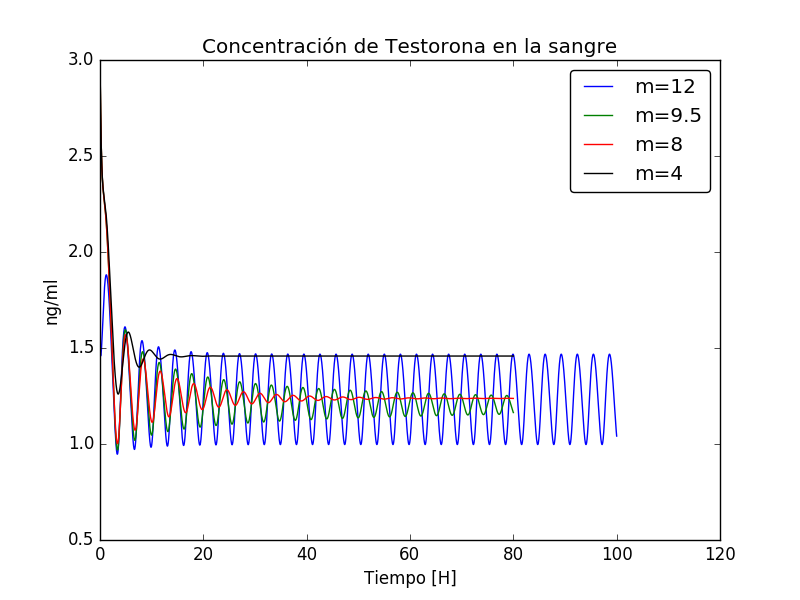
\includegraphics[width=3.5in]{imagenes/Graficas/Modelos_Simples/g1.png}
\end{center}
\end{frame}

\begin{frame}
\frametitle{Modelo Simple}
\begin{center}
 \includegraphics[width=3.5in]{imagenes/Graficas/Modelos_Simples/g2.png}
\end{center}
\end{frame}

\begin{frame}
\frametitle{Modelo Simple}
\begin{center}
 \includegraphics[width=3.5in]{imagenes/Graficas/Modelos_Simples/g3.png}
\end{center}
\end{frame}


\begin{frame}
\frametitle{Modelo Simple}
\begin{center}
 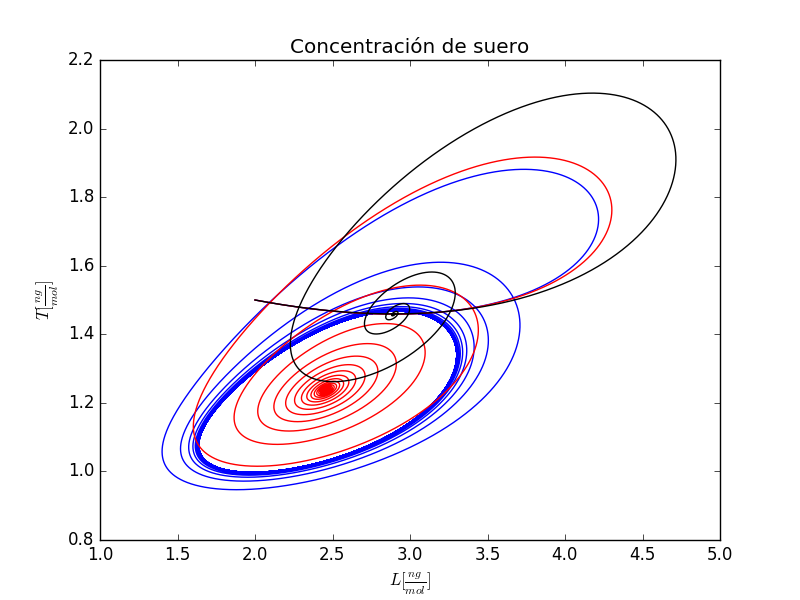
\includegraphics[width=3.5in]{imagenes/Graficas/Modelos_Simples/g4_2D.png}
\end{center}
\end{frame}

\begin{frame}
\frametitle{Modelo Simple}
\begin{center}
 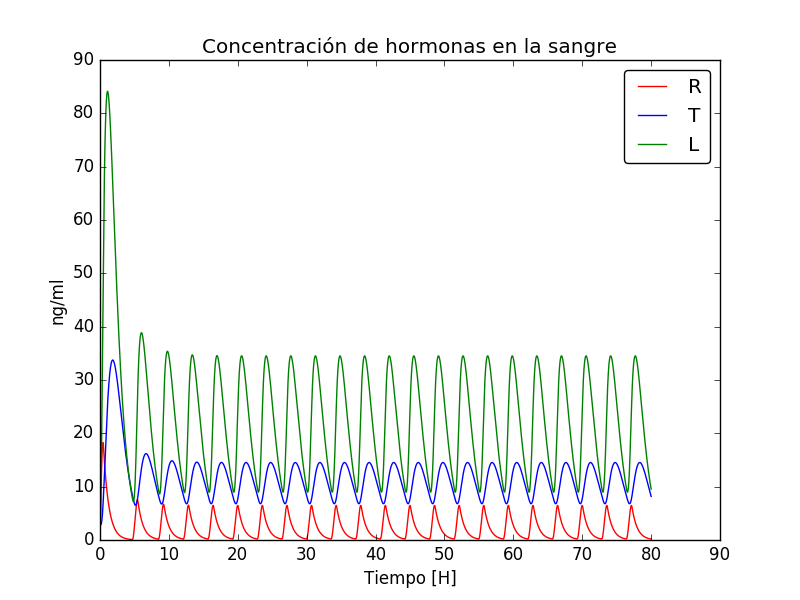
\includegraphics[width=3.5in]{imagenes/Graficas/Modelos_Simples/g5_g2-modelo2.png}
\end{center}
\end{frame}

\begin{frame}
\frametitle{Modelo Simple}
\begin{center}
 \includegraphics[width=3.5in]{imagenes/Graficas/Modelos_Simples/Comparacion_modelo_1_y_2.png}
\end{center}
\end{frame}

\subsection{Modelo con Fuente Externa}

\begin{frame}
\frametitle{Modelo con Fuente Externa}
En general, si se agregan fuentes constantes para las tres hormonas los valores en los que el sistema se deja de oscilar están descritos por:

$$ g_{1} g_{2} W_{R} + b_{1} g_{2} W_{L} + b_{1} b_{2} W_{T} > c b_{1} b_{2} b_{3} / h $$

Lo que arroja valores estacionarios:

$$ R_{o} = W_{R}/b_{1} $$

$$ L_{o} = \frac{g_{1} W_{R}/ b_{1} + W_{L}}{b_{2}}$$

$$ T_{o} = \dfrac{g_{1} g_{2} W_{R}/ b_{1} b_{2} + g_{2} W_{L}/b_{2} + W_{T}}{b_{3}}  $$


\end{frame}

\begin{frame}
\frametitle{Modelo con Fuente Externa}
\begin{center}
 \includegraphics[width=3.5in]{imagenes/Graficas/Modelo_fuente_externa-2/FE_modelo1_valor_critico_Wl.png}
\end{center}
\end{frame}


\begin{frame}
\frametitle{Modelo con Fuente Externa}
\begin{center}
 \includegraphics[width=3.5in]{imagenes/Graficas/Modelo_fuente_externa-2/FE_modelo1_valor_critico_Wt.png}
\end{center}
\end{frame}

\begin{frame}
\frametitle{Modelo con Fuente Externa}
\begin{center}
 \includegraphics[width=3.5in]{imagenes/Graficas/Modelo_fuente_externa-2/FE_modelo1_valor_no_critico_Wl.png}
\end{center}
\end{frame}


\begin{frame}
\frametitle{Modelo con Fuente Externa}
\begin{center}
 \includegraphics[width=3.5in]{imagenes/Graficas/Modelo_fuente_externa-2/FE_modelo1_valor_no_critico_Wt.png}
\end{center}
\end{frame}


\begin{frame}
\frametitle{Modelo con Fuente Externa}
\begin{center}
 \includegraphics[width=3.5in]{imagenes/Graficas/Modelo_fuente_externa-2/FE_modelo1_concentracion_de_suero_Wt.png}
\end{center}
\end{frame}

\begin{frame}
\frametitle{Modelo con Fuente Externa}
\begin{center}
 \includegraphics[width=3.5in]{imagenes/Graficas/Modelo_fuente_externa-2/FE_modelo2_valor_critico_Wl.png}
\end{center}
\end{frame}


\begin{frame}
\frametitle{Modelo con Fuente Externa}
\begin{center}
 \includegraphics[width=3.5in]{imagenes/Graficas/Modelo_fuente_externa-2/FE_modelo2_valor_critico_Wt.png}
\end{center}
\end{frame}

\begin{frame}
\frametitle{Modelo con Fuente Externa}
\begin{center}
 \includegraphics[width=3.5in]{imagenes/Graficas/Modelo_fuente_externa-2/FE_modelo2_valor_no_critico_Wl.png}
\end{center}
\end{frame}


\begin{frame}
\frametitle{Modelo con Fuente Externa}
\begin{center}
 \includegraphics[width=3.5in]{imagenes/Graficas/Modelo_fuente_externa-2/FE_modelo2_valor_no_critico_Wt.png}
\end{center}
\end{frame}


\subsection{Modelo de Castración}

\begin{frame}
\frametitle{Modelo de Castración}
\begin{center}
 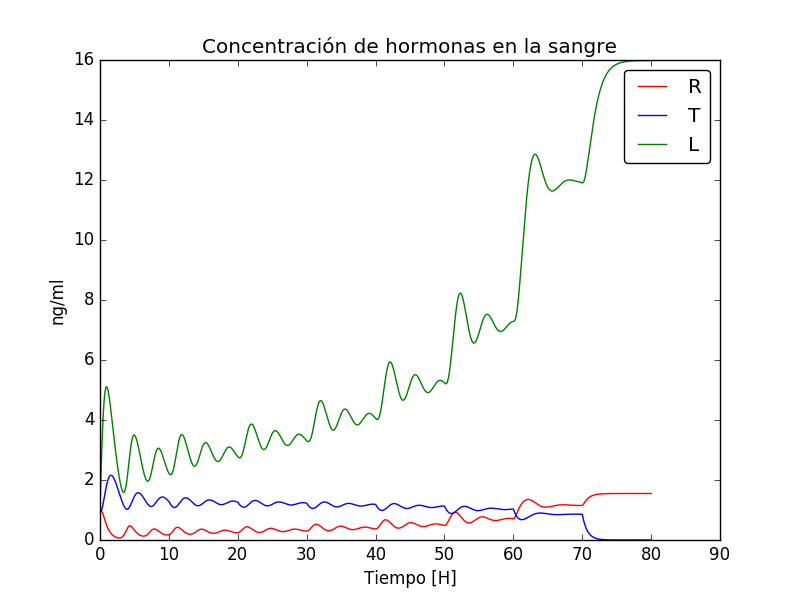
\includegraphics[width=3.5in]{imagenes/Graficas/Castracion/castracion_hormonas_primer_modelo_m_8.png}
\end{center}
\end{frame}

\begin{frame}
\frametitle{Modelo de Castración}
\begin{center}
 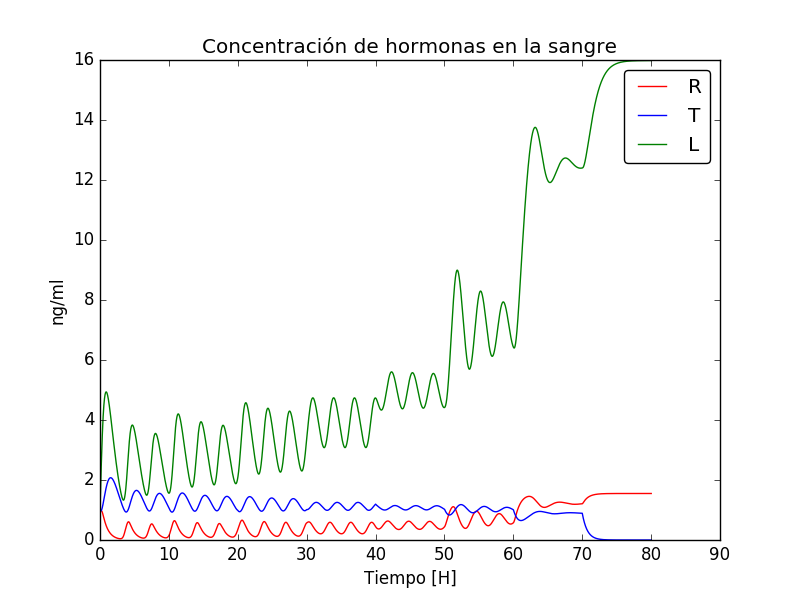
\includegraphics[width=3.5in]{imagenes/Graficas/Castracion/castracion_hormonas_primer_modelo_m_12.png}
\end{center}
\end{frame}

\begin{frame}
\frametitle{Modelo de Castración}
\begin{center}
 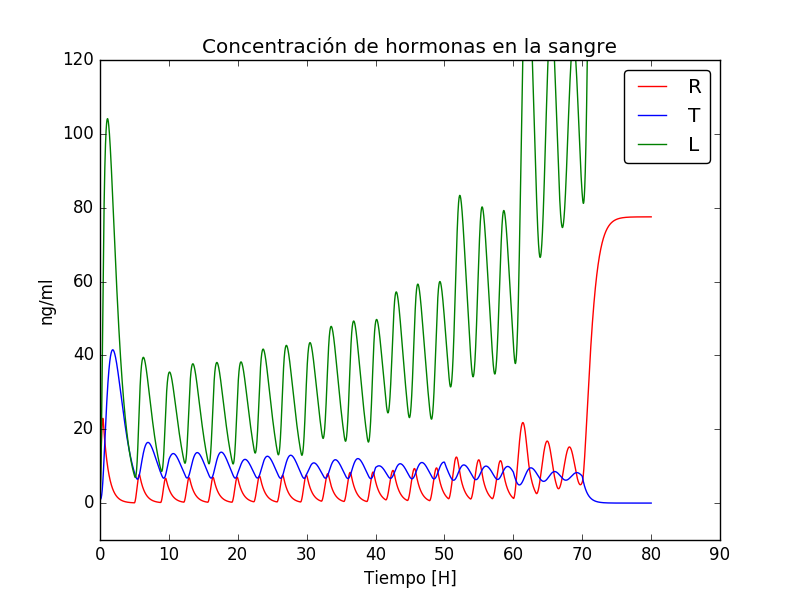
\includegraphics[width=3.5in]{imagenes/Graficas/Castracion/castracion_hormonas_segundo_modelo.png}
\end{center}
\end{frame}

\begin{frame}
\frametitle{Modelo de Castración}
\begin{center}
 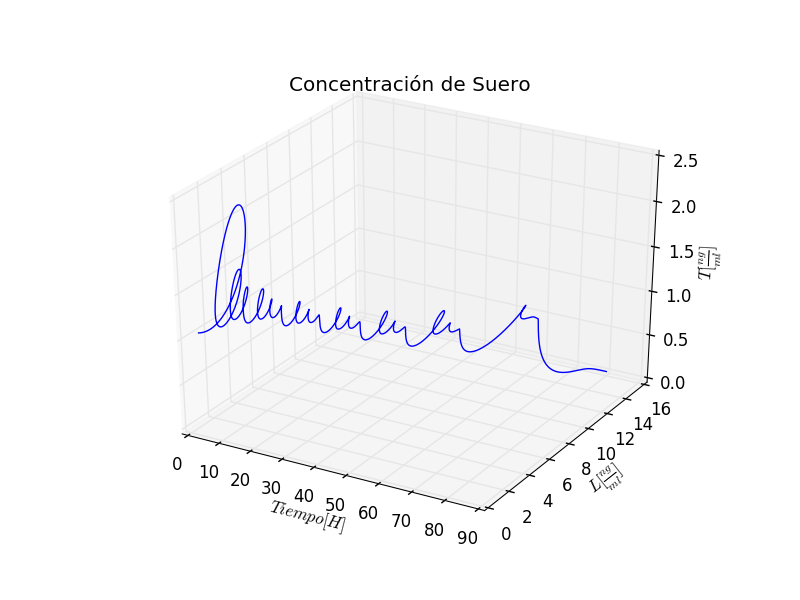
\includegraphics[width=3.5in]{imagenes/Graficas/Castracion/castracion_suero_primer_modelo_m_8.png}
\end{center}
\end{frame}

\begin{frame}
\frametitle{Modelo de Castración}
\begin{center}
 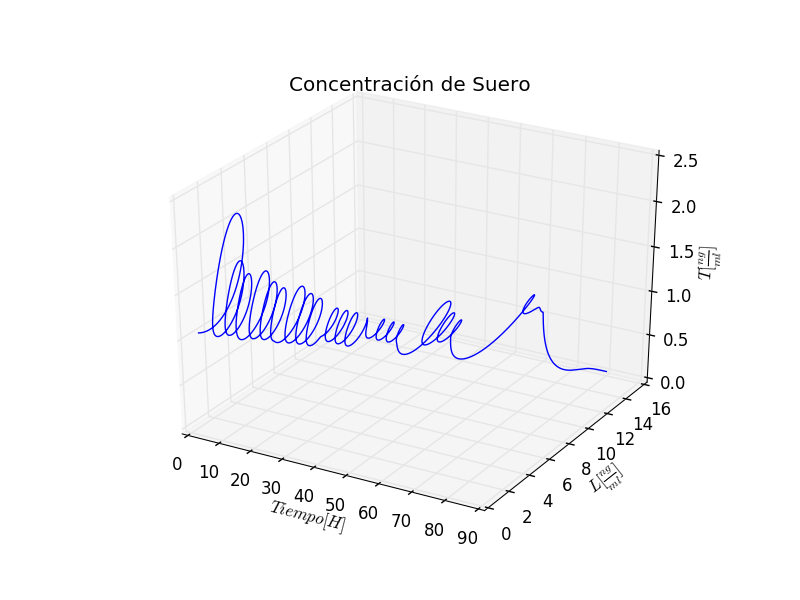
\includegraphics[width=3.5in]{imagenes/Graficas/Castracion/castracion_suero_primer_modelo_m_12.png}
\end{center}
\end{frame}

\begin{frame}
\frametitle{Modelo de Castración}
\begin{center}
 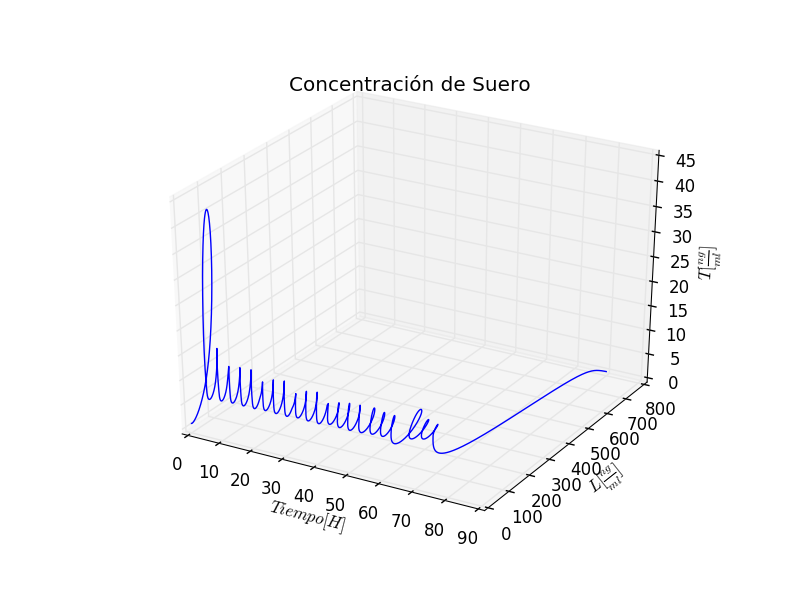
\includegraphics[width=3.5in]{imagenes/Graficas/Castracion/castracion_suero_segundo_modelo.png}
\end{center}
\end{frame}

\subsection{Pubertad}

\begin{frame}
\frametitle{Pubertad}

La pubertad está causada por uno o una combinación de los siguientes factores:\\

(i) Un incremento de la sensibilidad pituitaria para LHRH \\

Esto se representa con un incremento en g1

(ii) Un incremento de la sensibilidad gonadal para LH\\

Esto se representa con un incremento en g2

(iii) Un incremento de la sensibilidad hipotálamica hacia la retroalimentación negativa de la testosterona\\

Esto se representa con un incremento en h, dentro de la función f(T)

(iv) Un incremento en la tasa de secreción tónica de LHRH del hipotálamo\\

Esto se representa con un incremento en c, dentro de la función f(T)
\end{frame}

\begin{frame}
\frametitle{Modelo de Pubertad}
\begin{center}
 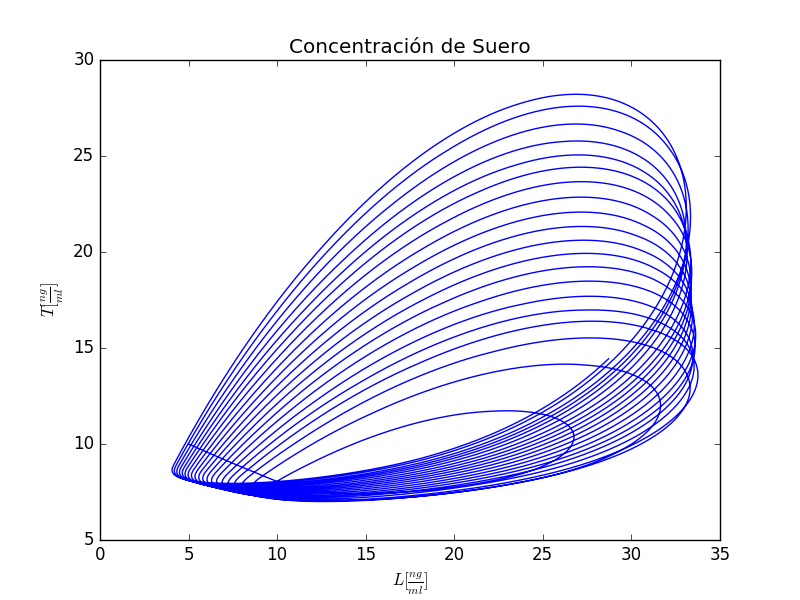
\includegraphics[width=3.5in]{imagenes/Graficas/Pubertad/pubertad_concentracion_de_suero.png}
\end{center}
\end{frame}

\begin{frame}
\frametitle{Modelo de Pubertad}
\begin{center}
 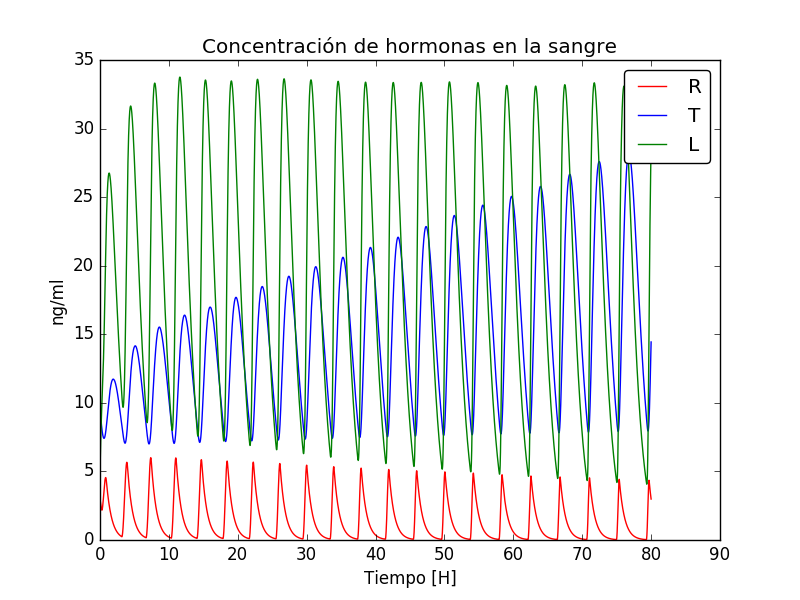
\includegraphics[width=3.5in]{imagenes/Graficas/Pubertad/pubertad.png}
\end{center}
\end{frame}

\begin{frame}
\frametitle{Conclusiones}
$\rightarrow$ Se encontraron valores críticos para Wt, Wr y Wl para el primer modelo.\\
$\rightarrow$ Se comprobaron númericamente los resultados propuestos por Smith.\\
$\rightarrow$ Se verificó que el estado estacionario del sistema no depende de las condiciones iniciales.\\
$\rightarrow$ Se logró modelar la castración y la pubertad para tiempo pequeños.\\
$\rightarrow$ Para poder describir adecuadamente la concentración de testosterona hay que incluir un retardo detro de la ecuación diferencial.\\
\end{frame}

\section{Referencias}
\begin{frame}
\frametitle{Referencias}
[1] Murray, J. D. 1989. Mathematical Biology. Volume 19. 

[2] Smith, William R. "Hypothalamic regulation of pituitary secretion of luteinizing hormone—II feedback control of gonadotropin secretion." Bulletin of Mathematical Biology 42.1 (1980): 57-78.
\end{frame}
\end{document}